\documentclass[fleqn]{book}
\usepackage[utf8]{inputenc}
\usepackage{../HBMath}
\usepackage{../Ceyhun}

\begin{document}

Şekil 2.3.3 de $Ç_1$ ve $Ç_2$ çizgeleri ile bu çizgelere
ilişkin çarpım çizge gösterilmiştir. Burada
örneğin, (11 , 21) ve (11 , 22) düğüm çifti için,
\[11=11 \quad ve \quad (21 , 22) \in \Psi \]
olduğundan, $Ç_1 \times Ç_2$ çizgesinde bu düğümler
bitişiktir.
\\
\begin{figure}[htb]
	\centering
	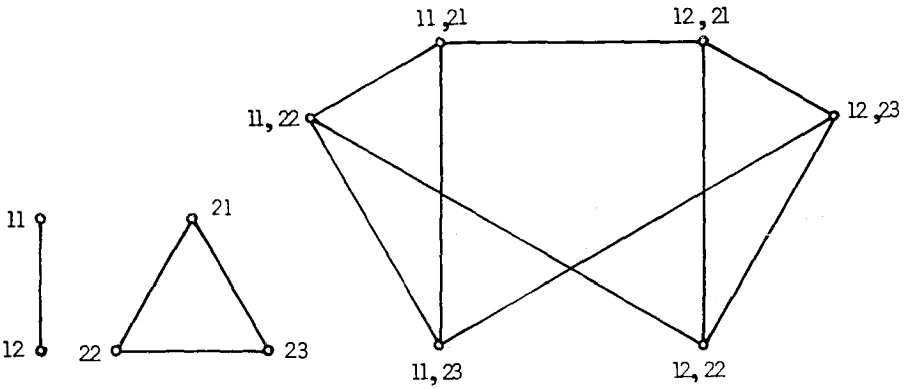
\includegraphics[width=0.9\textwidth]{images/ceyhun-68-fig01}
\end{figure}
\\
Şekil 2.3.3 $Ç_1$, $Ç_2$ ve ilişkin çarpım çizge $Ç_1 \times Ç_2$.
\begin{tanim}
	$Ç_1$, $Ç_2$ ve $Ç_1 [Ç_2]$ çizgelerinin
	düğüm ve ayrıt kümeleri sırasıyla,
	$\Delta_1, \Delta_2, \Delta_1 [\Delta_2]$  $\Psi_1, \Psi_2, \Psi_1 [\Psi_2]$
	olsun. Ayrıca
	$\Delta_1 \cap \Delta_2 \neq \emptyset$ koşulu sağlansın. Bu
	çizgelerin düğümlerini
	$d_{1_i} \in \Delta_1 \quad d_{2_j} \in \Delta_2$ ve \\
	$(d_{1_i}, d_{2_j}) \in \Delta_1 \times \Delta_2$
	olarak gösterelim. $Ç_1$in, $Ç_2$den
\end{tanim}

\end{document}